% Options for packages loaded elsewhere
\PassOptionsToPackage{unicode}{hyperref}
\PassOptionsToPackage{hyphens}{url}
%
\documentclass[
]{article}
\usepackage{amsmath,amssymb}
\usepackage{lmodern}
\usepackage{iftex}
\ifPDFTeX
  \usepackage[T1]{fontenc}
  \usepackage[utf8]{inputenc}
  \usepackage{textcomp} % provide euro and other symbols
\else % if luatex or xetex
  \usepackage{unicode-math}
  \defaultfontfeatures{Scale=MatchLowercase}
  \defaultfontfeatures[\rmfamily]{Ligatures=TeX,Scale=1}
\fi
% Use upquote if available, for straight quotes in verbatim environments
\IfFileExists{upquote.sty}{\usepackage{upquote}}{}
\IfFileExists{microtype.sty}{% use microtype if available
  \usepackage[]{microtype}
  \UseMicrotypeSet[protrusion]{basicmath} % disable protrusion for tt fonts
}{}
\makeatletter
\@ifundefined{KOMAClassName}{% if non-KOMA class
  \IfFileExists{parskip.sty}{%
    \usepackage{parskip}
  }{% else
    \setlength{\parindent}{0pt}
    \setlength{\parskip}{6pt plus 2pt minus 1pt}}
}{% if KOMA class
  \KOMAoptions{parskip=half}}
\makeatother
\usepackage{xcolor}
\IfFileExists{xurl.sty}{\usepackage{xurl}}{} % add URL line breaks if available
\IfFileExists{bookmark.sty}{\usepackage{bookmark}}{\usepackage{hyperref}}
\hypersetup{
  pdftitle={ADPS 2022Z --- Laboratorium 2 (rozwiązania)},
  pdfauthor={Adam Pruszyński},
  hidelinks,
  pdfcreator={LaTeX via pandoc}}
\urlstyle{same} % disable monospaced font for URLs
\usepackage[margin=1in]{geometry}
\usepackage{color}
\usepackage{fancyvrb}
\newcommand{\VerbBar}{|}
\newcommand{\VERB}{\Verb[commandchars=\\\{\}]}
\DefineVerbatimEnvironment{Highlighting}{Verbatim}{commandchars=\\\{\}}
% Add ',fontsize=\small' for more characters per line
\usepackage{framed}
\definecolor{shadecolor}{RGB}{248,248,248}
\newenvironment{Shaded}{\begin{snugshade}}{\end{snugshade}}
\newcommand{\AlertTok}[1]{\textcolor[rgb]{0.94,0.16,0.16}{#1}}
\newcommand{\AnnotationTok}[1]{\textcolor[rgb]{0.56,0.35,0.01}{\textbf{\textit{#1}}}}
\newcommand{\AttributeTok}[1]{\textcolor[rgb]{0.77,0.63,0.00}{#1}}
\newcommand{\BaseNTok}[1]{\textcolor[rgb]{0.00,0.00,0.81}{#1}}
\newcommand{\BuiltInTok}[1]{#1}
\newcommand{\CharTok}[1]{\textcolor[rgb]{0.31,0.60,0.02}{#1}}
\newcommand{\CommentTok}[1]{\textcolor[rgb]{0.56,0.35,0.01}{\textit{#1}}}
\newcommand{\CommentVarTok}[1]{\textcolor[rgb]{0.56,0.35,0.01}{\textbf{\textit{#1}}}}
\newcommand{\ConstantTok}[1]{\textcolor[rgb]{0.00,0.00,0.00}{#1}}
\newcommand{\ControlFlowTok}[1]{\textcolor[rgb]{0.13,0.29,0.53}{\textbf{#1}}}
\newcommand{\DataTypeTok}[1]{\textcolor[rgb]{0.13,0.29,0.53}{#1}}
\newcommand{\DecValTok}[1]{\textcolor[rgb]{0.00,0.00,0.81}{#1}}
\newcommand{\DocumentationTok}[1]{\textcolor[rgb]{0.56,0.35,0.01}{\textbf{\textit{#1}}}}
\newcommand{\ErrorTok}[1]{\textcolor[rgb]{0.64,0.00,0.00}{\textbf{#1}}}
\newcommand{\ExtensionTok}[1]{#1}
\newcommand{\FloatTok}[1]{\textcolor[rgb]{0.00,0.00,0.81}{#1}}
\newcommand{\FunctionTok}[1]{\textcolor[rgb]{0.00,0.00,0.00}{#1}}
\newcommand{\ImportTok}[1]{#1}
\newcommand{\InformationTok}[1]{\textcolor[rgb]{0.56,0.35,0.01}{\textbf{\textit{#1}}}}
\newcommand{\KeywordTok}[1]{\textcolor[rgb]{0.13,0.29,0.53}{\textbf{#1}}}
\newcommand{\NormalTok}[1]{#1}
\newcommand{\OperatorTok}[1]{\textcolor[rgb]{0.81,0.36,0.00}{\textbf{#1}}}
\newcommand{\OtherTok}[1]{\textcolor[rgb]{0.56,0.35,0.01}{#1}}
\newcommand{\PreprocessorTok}[1]{\textcolor[rgb]{0.56,0.35,0.01}{\textit{#1}}}
\newcommand{\RegionMarkerTok}[1]{#1}
\newcommand{\SpecialCharTok}[1]{\textcolor[rgb]{0.00,0.00,0.00}{#1}}
\newcommand{\SpecialStringTok}[1]{\textcolor[rgb]{0.31,0.60,0.02}{#1}}
\newcommand{\StringTok}[1]{\textcolor[rgb]{0.31,0.60,0.02}{#1}}
\newcommand{\VariableTok}[1]{\textcolor[rgb]{0.00,0.00,0.00}{#1}}
\newcommand{\VerbatimStringTok}[1]{\textcolor[rgb]{0.31,0.60,0.02}{#1}}
\newcommand{\WarningTok}[1]{\textcolor[rgb]{0.56,0.35,0.01}{\textbf{\textit{#1}}}}
\usepackage{graphicx}
\makeatletter
\def\maxwidth{\ifdim\Gin@nat@width>\linewidth\linewidth\else\Gin@nat@width\fi}
\def\maxheight{\ifdim\Gin@nat@height>\textheight\textheight\else\Gin@nat@height\fi}
\makeatother
% Scale images if necessary, so that they will not overflow the page
% margins by default, and it is still possible to overwrite the defaults
% using explicit options in \includegraphics[width, height, ...]{}
\setkeys{Gin}{width=\maxwidth,height=\maxheight,keepaspectratio}
% Set default figure placement to htbp
\makeatletter
\def\fps@figure{htbp}
\makeatother
\setlength{\emergencystretch}{3em} % prevent overfull lines
\providecommand{\tightlist}{%
  \setlength{\itemsep}{0pt}\setlength{\parskip}{0pt}}
\setcounter{secnumdepth}{-\maxdimen} % remove section numbering
\ifLuaTeX
  \usepackage{selnolig}  % disable illegal ligatures
\fi

\title{ADPS 2022Z --- Laboratorium 2 (rozwiązania)}
\author{Adam Pruszyński}
\date{}

\begin{document}
\maketitle

\hypertarget{zadanie-1-1-pkt}{%
\section{Zadanie 1 (1 pkt)}\label{zadanie-1-1-pkt}}

\hypertarget{treux15bux107-zadania}{%
\subsection{Treść zadania}\label{treux15bux107-zadania}}

Rozkład Poissona jest często używany do modelowania ruchu ulicznego (o
małym natężeniu). Plik
\href{http://elektron.elka.pw.edu.pl/~mrupniew/adps/skrety.txt}{skrety.txt}
zawiera liczby pojazdów skręcających na pewnym skrzyżowaniu w prawo w
przeciągu trzystu 3-minutowych przedziałów czasu (dane zostały zebrane o
różnych porach dnia).

\begin{itemize}
\item
  Wczytaj dane za pomocą komendy scan(`skrety.txt').
\item
  Dopasuj do danych rozkład Poissona, tj. wyestymuj parametr \(\lambda\)
  rozkładu Poissona.
\item
  Metodą bootstrapu nieparametrycznego oszacuj odchylenie standardowe
  estymatora parametru \(\lambda\).
\item
  Sprawdź i opisz zgodność rozkładu o wyestymowanym parametrze
  \(\lambda\) z zarejestrowanymi danymi porównując graficznie empiryczną
  i teoretyczną funkcję prawdopodobieństwa. Użyj funkcji table()
  i~dpois() analogicznie jak w przykładzie 4 laboratorium 1.
\end{itemize}

\hypertarget{rozwiux105zanie}{%
\subsection{Rozwiązanie}\label{rozwiux105zanie}}

\begin{Shaded}
\begin{Highlighting}[]
\NormalTok{n }\OtherTok{=} \DecValTok{300}
\NormalTok{turns }\OtherTok{=} \FunctionTok{scan}\NormalTok{(}\StringTok{\textquotesingle{}http://elektron.elka.pw.edu.pl/\textasciitilde{}mrupniew/adps/skrety.txt\textquotesingle{}}\NormalTok{)}

\NormalTok{lambda }\OtherTok{=} \FunctionTok{mean}\NormalTok{(turns)}
\NormalTok{quiet }\OtherTok{=} \ConstantTok{TRUE} 
\end{Highlighting}
\end{Shaded}

Estymata parametru lambda wynosi 3.8

\begin{Shaded}
\begin{Highlighting}[]
\NormalTok{K }\OtherTok{=} \DecValTok{1000}
\NormalTok{boot\_res }\OtherTok{=} \FunctionTok{replicate}\NormalTok{(K, \{}
\NormalTok{  boot\_dane }\OtherTok{=} \FunctionTok{sample}\NormalTok{(turns, n, }\AttributeTok{replace =}\NormalTok{ T)}
  \FunctionTok{c}\NormalTok{(}\FunctionTok{mean}\NormalTok{(boot\_dane))}
\NormalTok{\})}
\NormalTok{sd\_lambda }\OtherTok{=} \FunctionTok{sd}\NormalTok{(boot\_res)}
\end{Highlighting}
\end{Shaded}

Odchylenie standardowe estymatora parametru lambda wynosi 0.1306562

\begin{Shaded}
\begin{Highlighting}[]
\NormalTok{Arg }\OtherTok{=} \DecValTok{0}\SpecialCharTok{:}\FunctionTok{max}\NormalTok{(turns)}
\NormalTok{Freq }\OtherTok{=} \FunctionTok{as.numeric}\NormalTok{(}\FunctionTok{table}\NormalTok{(}\FunctionTok{factor}\NormalTok{(turns))) }\SpecialCharTok{/}\NormalTok{ n}

\FunctionTok{plot}\NormalTok{(Freq }\SpecialCharTok{\textasciitilde{}}\NormalTok{ Arg, }\AttributeTok{type =} \StringTok{\textquotesingle{}h\textquotesingle{}}\NormalTok{, }\AttributeTok{col =} \StringTok{\textquotesingle{}blue\textquotesingle{}}\NormalTok{, }
     \AttributeTok{xlab =} \StringTok{\textquotesingle{}Liczba skrętów w prawo\textquotesingle{}}\NormalTok{, }\AttributeTok{ylab =} \StringTok{\textquotesingle{}f(x)\textquotesingle{}}\NormalTok{, }
     \AttributeTok{xlim =} \FunctionTok{c}\NormalTok{(}\DecValTok{0}\NormalTok{, }\FloatTok{12.5}\NormalTok{), }\AttributeTok{main =} \FunctionTok{paste0}\NormalTok{(}\StringTok{\textquotesingle{}Funkcja prawdopodobieństwa dla M = \textquotesingle{}}\NormalTok{, n))}

\FunctionTok{grid}\NormalTok{()}

\FunctionTok{points}\NormalTok{(Freq }\SpecialCharTok{\textasciitilde{}}\NormalTok{ Arg, }\AttributeTok{col =} \StringTok{\textquotesingle{}blue\textquotesingle{}}\NormalTok{)}

\FunctionTok{lines}\NormalTok{(}\FunctionTok{dpois}\NormalTok{(Arg, lambda) }\SpecialCharTok{\textasciitilde{}}\NormalTok{ Arg, }\AttributeTok{type =} \StringTok{\textquotesingle{}h\textquotesingle{}}\NormalTok{, }\AttributeTok{col =} \StringTok{\textquotesingle{}red\textquotesingle{}}\NormalTok{)}

\FunctionTok{points}\NormalTok{(}\FunctionTok{dpois}\NormalTok{(Arg, lambda) }\SpecialCharTok{\textasciitilde{}}\NormalTok{ Arg, }\AttributeTok{col =} \StringTok{\textquotesingle{}red\textquotesingle{}}\NormalTok{)}

\FunctionTok{legend}\NormalTok{(}\StringTok{\textquotesingle{}topright\textquotesingle{}}\NormalTok{, }\FunctionTok{c}\NormalTok{(}\StringTok{\textquotesingle{}empiryczna\textquotesingle{}}\NormalTok{, }\StringTok{\textquotesingle{}teoretyczna\textquotesingle{}}\NormalTok{),}
    \AttributeTok{col =} \FunctionTok{c}\NormalTok{(}\StringTok{\textquotesingle{}blue\textquotesingle{}}\NormalTok{, }\StringTok{\textquotesingle{}red\textquotesingle{}}\NormalTok{), }\AttributeTok{lwd =} \DecValTok{1}\NormalTok{)}
\end{Highlighting}
\end{Shaded}

\includegraphics{ADPS_L2_files/figure-latex/unnamed-chunk-4-1.pdf}

Funckja prawdopodobieństwa wyznaczona metodą teoretyczną pokrywa się z
funkcją wyznaczoną metodą empriczyną. W obydwu przypadkach auta skręcały
najczęsćiej trzykrotnie.

\hypertarget{zadanie-2-1-pkt}{%
\section{Zadanie 2 (1 pkt)}\label{zadanie-2-1-pkt}}

\hypertarget{treux15bux107-zadania-1}{%
\subsection{Treść zadania}\label{treux15bux107-zadania-1}}

\begin{itemize}
\item
  Dla wybranej jednej spółki notowanej na GPW oblicz wartości
  procentowych zmian najwyższych cen w~dniu (high) dla roku 2020 i
  wykreśl ich histogram.
\item
  Wyestymuj wartość średnią oraz wariancję procentowych zmian
  najwyższych cen w dniu dla wybranej spółki.
\item
  Na podstawie histogramu i wykresu funkcji gęstości prawdopodobieństwa
  wyznaczonej dla wystymowanych parametrów (wartość średnia i wariancja)
  zweryfikuj zgrubnie, czy możemy przyjąć, że procentowe zmiany
  najwyższych cen w dniu mają rozkład normalny.
\item
  Zakładając, że zmiany najwyższych cen w dniu mają rozkład normalny
  wyznacz 90\%, 95\% i 99\% przedziały ufności dla wartości średniej i
  wariancji procentowych zmian najwyższych cen w dniu dla wybranej
  spółki. Przeanalizuj wyniki uzyskane dla różnych przedziałów ufności.
\end{itemize}

\hypertarget{rozwiux105zanie-1}{%
\subsection{Rozwiązanie}\label{rozwiux105zanie-1}}

\begin{Shaded}
\begin{Highlighting}[]
\ControlFlowTok{if}\NormalTok{(}\SpecialCharTok{!}\FunctionTok{file.exists}\NormalTok{(}\StringTok{\textquotesingle{}mstall.zip\textquotesingle{}}\NormalTok{)) \{}
\FunctionTok{download.file}\NormalTok{(}\StringTok{\textquotesingle{}https://info.bossa.pl/pub/metastock/mstock/mstall.zip\textquotesingle{}}\NormalTok{,}\StringTok{\textquotesingle{}mstall.zip\textquotesingle{}}\NormalTok{)}
\NormalTok{\}}

\FunctionTok{unzip}\NormalTok{(}\StringTok{\textquotesingle{}mstall.zip\textquotesingle{}}\NormalTok{, }\AttributeTok{files =} \FunctionTok{c}\NormalTok{(}\StringTok{\textquotesingle{}PKNORLEN.mst\textquotesingle{}}\NormalTok{))}
\NormalTok{df\_PKNORLEN }\OtherTok{=} \FunctionTok{read.csv}\NormalTok{(}\StringTok{\textquotesingle{}PKNORLEN.mst\textquotesingle{}}\NormalTok{)}

\NormalTok{col\_names }\OtherTok{=} \FunctionTok{c}\NormalTok{(}\StringTok{\textquotesingle{}ticker\textquotesingle{}}\NormalTok{, }\StringTok{\textquotesingle{}date\textquotesingle{}}\NormalTok{, }\StringTok{\textquotesingle{}open\textquotesingle{}}\NormalTok{, }\StringTok{\textquotesingle{}high\textquotesingle{}}\NormalTok{, }\StringTok{\textquotesingle{}low\textquotesingle{}}\NormalTok{, }\StringTok{\textquotesingle{}close\textquotesingle{}}\NormalTok{,}\StringTok{\textquotesingle{}vol\textquotesingle{}}\NormalTok{)}
\FunctionTok{names}\NormalTok{(df\_PKNORLEN) }\OtherTok{=}\NormalTok{ col\_names}

\NormalTok{df\_PKNORLEN}\SpecialCharTok{$}\NormalTok{date }\OtherTok{=} \FunctionTok{as.Date.character}\NormalTok{(df\_PKNORLEN}\SpecialCharTok{$}\NormalTok{date, }\AttributeTok{format =}\StringTok{\textquotesingle{}\%Y\%m\%d\textquotesingle{}}\NormalTok{)}
\NormalTok{df\_PKNORLEN }\OtherTok{=}\NormalTok{ df\_PKNORLEN[}\FunctionTok{which}\NormalTok{(df\_PKNORLEN}\SpecialCharTok{$}\NormalTok{date }\SpecialCharTok{\textgreater{}=} \StringTok{\textquotesingle{}2020{-}01{-}01\textquotesingle{}} \SpecialCharTok{\&}\NormalTok{ df\_PKNORLEN}\SpecialCharTok{$}\NormalTok{date }\SpecialCharTok{\textless{}=} \StringTok{\textquotesingle{}2020{-}12{-}31\textquotesingle{}}\NormalTok{),]}

\NormalTok{df\_PKNORLEN}\SpecialCharTok{$}\NormalTok{high\_ch }\OtherTok{=} \FunctionTok{with}\NormalTok{(df\_PKNORLEN, }\FunctionTok{c}\NormalTok{(}\DecValTok{0}\NormalTok{, }\FunctionTok{round}\NormalTok{(}\DecValTok{100}\SpecialCharTok{*}\FunctionTok{diff}\NormalTok{(high)}\SpecialCharTok{/}\NormalTok{high[}\SpecialCharTok{{-}}\FunctionTok{length}\NormalTok{(high)], }\AttributeTok{digits =} \DecValTok{2}\NormalTok{)))}

\NormalTok{high\_ch\_mean }\OtherTok{=} \FunctionTok{mean}\NormalTok{(df\_PKNORLEN}\SpecialCharTok{$}\NormalTok{high\_ch, }\AttributeTok{na.rm =}\NormalTok{ T)}
\NormalTok{high\_ch\_sd }\OtherTok{=} \FunctionTok{sd}\NormalTok{(df\_PKNORLEN}\SpecialCharTok{$}\NormalTok{high\_ch, }\AttributeTok{na.rm =}\NormalTok{ T)}
\NormalTok{high\_ch\_var }\OtherTok{=} \FunctionTok{var}\NormalTok{(df\_PKNORLEN}\SpecialCharTok{$}\NormalTok{high\_ch, }\AttributeTok{na.rm =}\NormalTok{ T)}

\FunctionTok{hist}\NormalTok{(df\_PKNORLEN}\SpecialCharTok{$}\NormalTok{high\_ch, }\AttributeTok{breaks =} \DecValTok{50}\NormalTok{, }\AttributeTok{prob =}\NormalTok{ T, }
     \AttributeTok{col =} \StringTok{\textquotesingle{}red\textquotesingle{}}\NormalTok{, }\AttributeTok{xlab =} \StringTok{\textquotesingle{}Zmiana najwyższej ceny w dniu [\%]\textquotesingle{}}\NormalTok{,}
     \AttributeTok{ylab =} \StringTok{\textquotesingle{}Częstość występowania\textquotesingle{}}\NormalTok{, }
     \AttributeTok{main =} \StringTok{\textquotesingle{}Histogram procentowych zmian najwyższych cen }\SpecialCharTok{\textbackslash{}n}\StringTok{  dla PKN ORLEN w 2020 roku\textquotesingle{}}\NormalTok{)}

\FunctionTok{grid}\NormalTok{()}

\NormalTok{min\_c }\OtherTok{=} \FunctionTok{min}\NormalTok{(df\_PKNORLEN}\SpecialCharTok{$}\NormalTok{high\_ch, }\AttributeTok{na.rm =}\NormalTok{ T)}
\NormalTok{max\_c }\OtherTok{=} \FunctionTok{max}\NormalTok{(df\_PKNORLEN}\SpecialCharTok{$}\NormalTok{high\_ch, }\AttributeTok{na.rm =}\NormalTok{ T)}

\FunctionTok{curve}\NormalTok{(}\FunctionTok{dnorm}\NormalTok{(x, }\AttributeTok{mean =}\NormalTok{ high\_ch\_mean,}
\AttributeTok{sd =}\NormalTok{ high\_ch\_sd), }\AttributeTok{add =}\NormalTok{ T, }\AttributeTok{col =} \StringTok{\textquotesingle{}blue\textquotesingle{}}\NormalTok{, }\AttributeTok{from =}\NormalTok{ min\_c, }\AttributeTok{to =}\NormalTok{ max\_c)}
\end{Highlighting}
\end{Shaded}

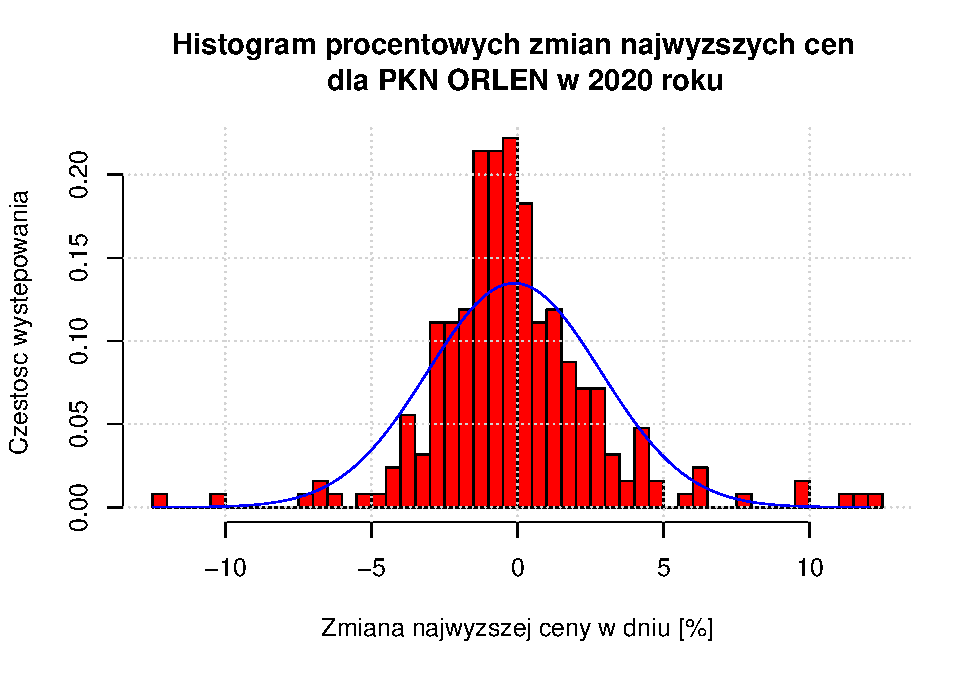
\includegraphics{ADPS_L2_files/figure-latex/unnamed-chunk-5-1.pdf}
Wyestymowana wartość średniej wynosi -0.1100794, natomiast wariancji
8.7564119.

Procentowe zmiany najwyższych cen w dniu mają rozkład normalny, ponieważ
naniesiona krzywa funkcji gęstości jest zbliżona do narysowanego
historgramu. Maksimum występuję mniej więcej w tym samym miejscu tzn w
punkcie -0.11.

\begin{Shaded}
\begin{Highlighting}[]
\NormalTok{n }\OtherTok{=} \FunctionTok{length}\NormalTok{(df\_PKNORLEN}\SpecialCharTok{$}\NormalTok{high\_ch)}
\NormalTok{S }\OtherTok{=}\NormalTok{ high\_ch\_sd}

\NormalTok{lev90 }\OtherTok{=} \FloatTok{0.9}
\NormalTok{w90 }\OtherTok{=}\NormalTok{ S}\SpecialCharTok{*}\FunctionTok{qt}\NormalTok{((}\DecValTok{1}\SpecialCharTok{+}\NormalTok{lev90)}\SpecialCharTok{/}\DecValTok{2}\NormalTok{, n}\DecValTok{{-}1}\NormalTok{)}\SpecialCharTok{/}\FunctionTok{sqrt}\NormalTok{(n)}
\NormalTok{ci\_mean\_90 }\OtherTok{=} \FunctionTok{c}\NormalTok{(high\_ch\_mean }\SpecialCharTok{{-}}\NormalTok{ w90, high\_ch\_mean }\SpecialCharTok{+}\NormalTok{ w90)}
\NormalTok{a }\OtherTok{=}\NormalTok{ (}\DecValTok{1} \SpecialCharTok{{-}}\NormalTok{ lev90)}\SpecialCharTok{/}\DecValTok{2}\NormalTok{; b }\OtherTok{=}\NormalTok{ (}\DecValTok{1} \SpecialCharTok{{-}}\NormalTok{ lev90)}\SpecialCharTok{/}\DecValTok{2}
\NormalTok{ci\_var\_90 }\OtherTok{=} \FunctionTok{c}\NormalTok{((n}\DecValTok{{-}1}\NormalTok{)}\SpecialCharTok{*}\NormalTok{S}\SpecialCharTok{\^{}}\DecValTok{2}\SpecialCharTok{/}\FunctionTok{qchisq}\NormalTok{(}\DecValTok{1}\SpecialCharTok{{-}}\NormalTok{b,n}\DecValTok{{-}1}\NormalTok{), (n}\DecValTok{{-}1}\NormalTok{)}\SpecialCharTok{*}\NormalTok{S}\SpecialCharTok{\^{}}\DecValTok{2}\SpecialCharTok{/}\FunctionTok{qchisq}\NormalTok{(a,n}\DecValTok{{-}1}\NormalTok{))}
\end{Highlighting}
\end{Shaded}

Granice 90 \% przedziału ufności dla wartosci średniej wynoszą:
-0.4178279, 0.1976691.

Granice 90 \% przedziału ufności dla wariancji wynoszą 7.6062326,
10.2075035

\begin{Shaded}
\begin{Highlighting}[]
\NormalTok{lev95 }\OtherTok{=} \FloatTok{0.95}
\NormalTok{w95 }\OtherTok{=}\NormalTok{ S}\SpecialCharTok{*}\FunctionTok{qt}\NormalTok{((}\DecValTok{1}\SpecialCharTok{+}\NormalTok{lev95)}\SpecialCharTok{/}\DecValTok{2}\NormalTok{, n}\DecValTok{{-}1}\NormalTok{)}\SpecialCharTok{/}\FunctionTok{sqrt}\NormalTok{(n)}
\NormalTok{ci\_mean\_95 }\OtherTok{=} \FunctionTok{c}\NormalTok{(high\_ch\_mean }\SpecialCharTok{{-}}\NormalTok{ w95, high\_ch\_mean }\SpecialCharTok{+}\NormalTok{ w95)}
\NormalTok{a }\OtherTok{=}\NormalTok{ (}\DecValTok{1} \SpecialCharTok{{-}}\NormalTok{ lev95)}\SpecialCharTok{/}\DecValTok{2}\NormalTok{; b }\OtherTok{=}\NormalTok{ (}\DecValTok{1} \SpecialCharTok{{-}}\NormalTok{ lev95)}\SpecialCharTok{/}\DecValTok{2}
\NormalTok{ci\_var\_95 }\OtherTok{=} \FunctionTok{c}\NormalTok{((n}\DecValTok{{-}1}\NormalTok{)}\SpecialCharTok{*}\NormalTok{S}\SpecialCharTok{\^{}}\DecValTok{2}\SpecialCharTok{/}\FunctionTok{qchisq}\NormalTok{(}\DecValTok{1}\SpecialCharTok{{-}}\NormalTok{b,n}\DecValTok{{-}1}\NormalTok{), (n}\DecValTok{{-}1}\NormalTok{)}\SpecialCharTok{*}\NormalTok{S}\SpecialCharTok{\^{}}\DecValTok{2}\SpecialCharTok{/}\FunctionTok{qchisq}\NormalTok{(a,n}\DecValTok{{-}1}\NormalTok{))}
\end{Highlighting}
\end{Shaded}

Granice 95 \% przedziału ufności dla wartosci średniej wynoszą:
-0.477201, 0.2570423.

Granice 95 \% przedziału ufności dla wariancji wynoszą 7.4057791,
10.5155616.

\begin{Shaded}
\begin{Highlighting}[]
\NormalTok{lev99 }\OtherTok{=} \FloatTok{0.99}
\NormalTok{w99 }\OtherTok{=}\NormalTok{ S}\SpecialCharTok{*}\FunctionTok{qt}\NormalTok{((}\DecValTok{1}\SpecialCharTok{+}\NormalTok{lev99)}\SpecialCharTok{/}\DecValTok{2}\NormalTok{, n}\DecValTok{{-}1}\NormalTok{)}\SpecialCharTok{/}\FunctionTok{sqrt}\NormalTok{(n)}
\NormalTok{ci\_mean\_99 }\OtherTok{=} \FunctionTok{c}\NormalTok{(high\_ch\_mean }\SpecialCharTok{{-}}\NormalTok{ w99, high\_ch\_mean }\SpecialCharTok{+}\NormalTok{ w99)}
\NormalTok{a }\OtherTok{=}\NormalTok{ (}\DecValTok{1} \SpecialCharTok{{-}}\NormalTok{ lev99)}\SpecialCharTok{/}\DecValTok{2}\NormalTok{; b }\OtherTok{=}\NormalTok{ (}\DecValTok{1} \SpecialCharTok{{-}}\NormalTok{ lev99)}\SpecialCharTok{/}\DecValTok{2}
\NormalTok{ci\_var\_99 }\OtherTok{=} \FunctionTok{c}\NormalTok{((n}\DecValTok{{-}1}\NormalTok{)}\SpecialCharTok{*}\NormalTok{S}\SpecialCharTok{\^{}}\DecValTok{2}\SpecialCharTok{/}\FunctionTok{qchisq}\NormalTok{(}\DecValTok{1}\SpecialCharTok{{-}}\NormalTok{b,n}\DecValTok{{-}1}\NormalTok{), (n}\DecValTok{{-}1}\NormalTok{)}\SpecialCharTok{*}\NormalTok{S}\SpecialCharTok{\^{}}\DecValTok{2}\SpecialCharTok{/}\FunctionTok{qchisq}\NormalTok{(a,n}\DecValTok{{-}1}\NormalTok{))}
\end{Highlighting}
\end{Shaded}

Granice 99 \% przedziału ufności dla wartosci średniej wynoszą:
-0.5939102, 0.3737515.

Granice 99 \% przedziału ufności dla wariancji wynoszą 7.0340221,
11.154069.

Im większy poziom ufności zastosujemy, tym szerszy otrzymamy przedział
zarówno dla średniej, jak i wariancji.

\begin{center}\rule{0.5\linewidth}{0.5pt}\end{center}

\hypertarget{zadanie-3-15-pkt.}{%
\section{Zadanie 3 (1,5 pkt.)}\label{zadanie-3-15-pkt.}}

\hypertarget{treux15bux107-zadania-2}{%
\subsection{Treść zadania}\label{treux15bux107-zadania-2}}

Rzucona pinezka upada ostrzem do dołu lub do góry. Doświadczenie to
można opisać rozkładem Bernoulliego z parametrem \(p\) będącym
prawdopodobieństwem tego, że pinezka upadnie ostrzem do góry.

Rozkład parametru \(p\) można opisać rozkładem beta o parametrach
\(\alpha\) i \(\beta\). Wartość średnia i wariancja w~rozkładzie beta
zależą od parametrów rozkładu w następujący sposób:
\[ \mathbb{E}X = \frac{\alpha}{\alpha + \beta}, \qquad \mathbb{V}X = \frac{\alpha\beta}{(\alpha + \beta)^2(\alpha + \beta + 1)}, \qquad dominanta = \frac{\alpha - 1}{\alpha + \beta - 2}.\]

\begin{itemize}
\item
  Na podstawie przypuszczanej (a priori) wartości oczekiwanej parametru
  \(p\) zaproponuj wartości parametrów \(\alpha\) i \(\beta\) rozkładu a
  priori parametru \(p\). Narysuj rozkład a priori parametru \(p\)
  (wykorzystaj funkcję dbeta()).
\item
  Rzuć pinezką 20 razy i zanotuj wyniki kolejnych rzutów (1 - pinezka
  upada ostrzem do góry, 0 - pinezka upada ostrzem do dołu). Wyznacz i
  narysuj rozkład a posteriori parametru \(p\) oraz oblicz wartość
  bayesowskiego estymatora \(\hat{p}\). W~rozważanym przypadku rozkład
  aposteriori parametru \(p\) jest również rozkładem beta o parametrach:
  \[ \alpha_{\textrm{post}} = \alpha_{\textrm{prior}} + \sum_{i=1}^n x_i, \qquad \beta_{\textrm{post}} = \beta_{\textrm{prior}} + n - \sum_{i=1}^n x_i,\qquad x_i\in\{0,1\}.\]
\item
  Rzuć pinezką jeszcze 20 razy i zanotuj wyniki. Wyznacz i narysuj
  rozkład a posteriori oparty na wszystkich 40 rzutach oraz oblicz
  wartość bayesowskiego estymatora \(\hat{p}\) w tym przypadku. Porównaj
  wyniki z wynikami uzyskanymi po pierwszych 20 rzutach.
\item
  Korzystając ze wzoru na wariancję rozkładu Beta wyznacz i porównaj
  wariancje rozkładu a priori, a~posteriori po 20 rzutach i a posteriori
  po 40 rzutach.
\end{itemize}

\hypertarget{rozwiux105zanie-2}{%
\subsection{Rozwiązanie}\label{rozwiux105zanie-2}}

Flanki - gra zespołowa, polegająca na próbie trafienia czymkolwiek w
pustą puszkę stojącą po 3 metry od obu drużyn. Gdy puszka zostanie
przewrócona, drużyna która tego dokonała pije piwo ``na hejnał'', a
przeciwnik musi jak najszybciej podnieść przewróconą puszkę, wbiec z
powrotem za linie, gdy przekroczymy linie krzyczymy stop, a przeciwna
drużyna przestaje pić. Przyjmujemy, że strącenie puszki to 1, a
chybienie - 0. Prawdopodobieństwo szacujemy na p = 0.2. Alfa i beta
przyjmujemy ze wzoru powyżej.

\begin{Shaded}
\begin{Highlighting}[]
\NormalTok{p }\OtherTok{=} \FloatTok{0.2}
\NormalTok{alpha\_priori }\OtherTok{=} \DecValTok{2}
\NormalTok{beta\_priori }\OtherTok{=} \DecValTok{8}

\NormalTok{a\_priori }\OtherTok{=}\NormalTok{ alpha\_priori }\SpecialCharTok{*}\NormalTok{ beta\_priori}
\NormalTok{b\_priori }\OtherTok{=}\NormalTok{ (alpha\_priori }\SpecialCharTok{+}\NormalTok{ beta\_priori)}\SpecialCharTok{\^{}}\DecValTok{2}
\NormalTok{c\_priori }\OtherTok{=}\NormalTok{ alpha\_priori }\SpecialCharTok{+}\NormalTok{ beta\_priori }\SpecialCharTok{+} \DecValTok{1}

\NormalTok{var\_priori }\OtherTok{=}\NormalTok{ a\_priori }\SpecialCharTok{/}\NormalTok{ (b\_priori }\SpecialCharTok{*}\NormalTok{ c\_priori)}
\end{Highlighting}
\end{Shaded}

Wykonano 20 rzutów. Wyniki to 2 trafienia w puszkę, 18 chybień.
Obliczamy a posteriori alfę i betę zgodnie z tabelą w wykładu.

\begin{Shaded}
\begin{Highlighting}[]
\NormalTok{hit\_round\_1 }\OtherTok{=} \DecValTok{2}
\NormalTok{missed\_round\_1 }\OtherTok{=} \DecValTok{18}

\NormalTok{alpha\_round\_1 }\OtherTok{=}\NormalTok{ alpha\_priori }\SpecialCharTok{+}\NormalTok{ hit\_round\_1}
\NormalTok{beta\_round\_1 }\OtherTok{=}\NormalTok{ beta\_priori }\SpecialCharTok{+}\NormalTok{ missed\_round\_1}

\NormalTok{p\_round\_1 }\OtherTok{=}\NormalTok{ alpha\_round\_1 }\SpecialCharTok{/}\NormalTok{ (alpha\_round\_1 }\SpecialCharTok{+}\NormalTok{ beta\_round\_1)}

\NormalTok{a\_round\_1 }\OtherTok{=}\NormalTok{ alpha\_round\_1 }\SpecialCharTok{*}\NormalTok{ beta\_round\_1}
\NormalTok{b\_round\_1 }\OtherTok{=}\NormalTok{ (alpha\_round\_1 }\SpecialCharTok{+}\NormalTok{ beta\_round\_1)}\SpecialCharTok{\^{}}\DecValTok{2}
\NormalTok{c\_round\_1 }\OtherTok{=}\NormalTok{ alpha\_round\_1 }\SpecialCharTok{+}\NormalTok{ beta\_round\_1 }\SpecialCharTok{+} \DecValTok{1}

\NormalTok{var\_round\_1 }\OtherTok{=}\NormalTok{ a\_round\_1 }\SpecialCharTok{/}\NormalTok{ (b\_round\_1 }\SpecialCharTok{*}\NormalTok{ c\_round\_1)}
\end{Highlighting}
\end{Shaded}

W drugiej rundzie flanek uczestnicy wykonali kolejne 20 rzutów. Puszkę
strącono 4 razy.

\begin{Shaded}
\begin{Highlighting}[]
\NormalTok{hit\_round\_2 }\OtherTok{=} \DecValTok{4}
\NormalTok{missed\_round\_2 }\OtherTok{=} \DecValTok{16}

\NormalTok{alpha\_round\_2 }\OtherTok{=}\NormalTok{ alpha\_round\_1 }\SpecialCharTok{+}\NormalTok{ hit\_round\_2}
\NormalTok{beta\_round\_2 }\OtherTok{=}\NormalTok{ beta\_round\_1 }\SpecialCharTok{+}\NormalTok{ missed\_round\_2}

\NormalTok{p\_round\_2 }\OtherTok{=}\NormalTok{ alpha\_round\_2 }\SpecialCharTok{/}\NormalTok{ (alpha\_round\_2 }\SpecialCharTok{+}\NormalTok{ beta\_round\_2)}

\NormalTok{a\_round\_2 }\OtherTok{=}\NormalTok{ alpha\_round\_2 }\SpecialCharTok{*}\NormalTok{ beta\_round\_2}
\NormalTok{b\_round\_2 }\OtherTok{=}\NormalTok{ (alpha\_round\_2 }\SpecialCharTok{+}\NormalTok{ beta\_round\_2)}\SpecialCharTok{\^{}}\DecValTok{2}
\NormalTok{c\_round\_2 }\OtherTok{=}\NormalTok{ alpha\_round\_2 }\SpecialCharTok{+}\NormalTok{ beta\_round\_2 }\SpecialCharTok{+} \DecValTok{1}

\NormalTok{var\_round\_2 }\OtherTok{=}\NormalTok{ a\_round\_2 }\SpecialCharTok{/}\NormalTok{ (b\_round\_2 }\SpecialCharTok{*}\NormalTok{ c\_round\_2)}
\end{Highlighting}
\end{Shaded}

Rykres rozkładów a priori oraz a posteriori po dwóch rundach flanek.

\begin{Shaded}
\begin{Highlighting}[]
\FunctionTok{curve}\NormalTok{(}\FunctionTok{dbeta}\NormalTok{(x, }\AttributeTok{shape1 =}\NormalTok{ alpha\_priori, }\AttributeTok{shape2 =}\NormalTok{ beta\_priori),}
      \AttributeTok{lwd =} \FloatTok{1.5}\NormalTok{, }\AttributeTok{col =} \StringTok{\textquotesingle{}red\textquotesingle{}}\NormalTok{, }\AttributeTok{xlab =} \StringTok{\textquotesingle{}x\textquotesingle{}}\NormalTok{, }\AttributeTok{ylab =} \StringTok{\textquotesingle{}f(x)\textquotesingle{}}\NormalTok{,}
      \AttributeTok{main =} \StringTok{\textquotesingle{}Rozkład\textquotesingle{}}\NormalTok{, }\AttributeTok{xlim =} \FunctionTok{c}\NormalTok{(}\DecValTok{0}\NormalTok{, }\FloatTok{0.8}\NormalTok{), }\AttributeTok{ylim =} \FunctionTok{c}\NormalTok{(}\DecValTok{0}\NormalTok{, }\FloatTok{8.5}\NormalTok{))}

\FunctionTok{curve}\NormalTok{(}\FunctionTok{dbeta}\NormalTok{(x, }\AttributeTok{shape1 =}\NormalTok{ alpha\_round\_1, }\AttributeTok{shape2 =}\NormalTok{ beta\_round\_1),}
      \AttributeTok{add =} \ConstantTok{TRUE}\NormalTok{, }\AttributeTok{lwd =} \FloatTok{1.5}\NormalTok{, }\AttributeTok{col =} \StringTok{\textquotesingle{}blue\textquotesingle{}}\NormalTok{, }\AttributeTok{xlim =} \FunctionTok{c}\NormalTok{(}\DecValTok{0}\NormalTok{, }\FloatTok{0.8}\NormalTok{),}
      \AttributeTok{ylim =} \FunctionTok{c}\NormalTok{(}\DecValTok{0}\NormalTok{, }\FloatTok{8.5}\NormalTok{))}

\FunctionTok{curve}\NormalTok{(}\FunctionTok{dbeta}\NormalTok{(x, }\AttributeTok{shape1 =}\NormalTok{ alpha\_round\_2, }\AttributeTok{shape2 =}\NormalTok{ beta\_round\_2), }\AttributeTok{add =} \ConstantTok{TRUE}\NormalTok{,}
      \AttributeTok{lwd =} \FloatTok{1.5}\NormalTok{, }\AttributeTok{col =} \StringTok{\textquotesingle{}green\textquotesingle{}}\NormalTok{, }\AttributeTok{xlim =} \FunctionTok{c}\NormalTok{(}\DecValTok{0}\NormalTok{, }\FloatTok{0.8}\NormalTok{), }\AttributeTok{ylim =} \FunctionTok{c}\NormalTok{(}\DecValTok{0}\NormalTok{, }\FloatTok{8.5}\NormalTok{))}

\FunctionTok{legend}\NormalTok{(}\StringTok{\textquotesingle{}topright\textquotesingle{}}\NormalTok{, }\FunctionTok{c}\NormalTok{(}\StringTok{\textquotesingle{}A priori\textquotesingle{}}\NormalTok{, }\StringTok{\textquotesingle{}A posteriori po 1 rundzie flanek\textquotesingle{}}\NormalTok{,}
      \StringTok{\textquotesingle{}A posteriori po 2 rundzie flanek\textquotesingle{}}\NormalTok{), }\AttributeTok{col =} \FunctionTok{c}\NormalTok{(}\StringTok{\textquotesingle{}red\textquotesingle{}}\NormalTok{, }\StringTok{\textquotesingle{}blue\textquotesingle{}}\NormalTok{, }\StringTok{\textquotesingle{}green\textquotesingle{}}\NormalTok{), }\AttributeTok{lwd =} \DecValTok{2}\NormalTok{)}

\FunctionTok{grid}\NormalTok{()}
\end{Highlighting}
\end{Shaded}

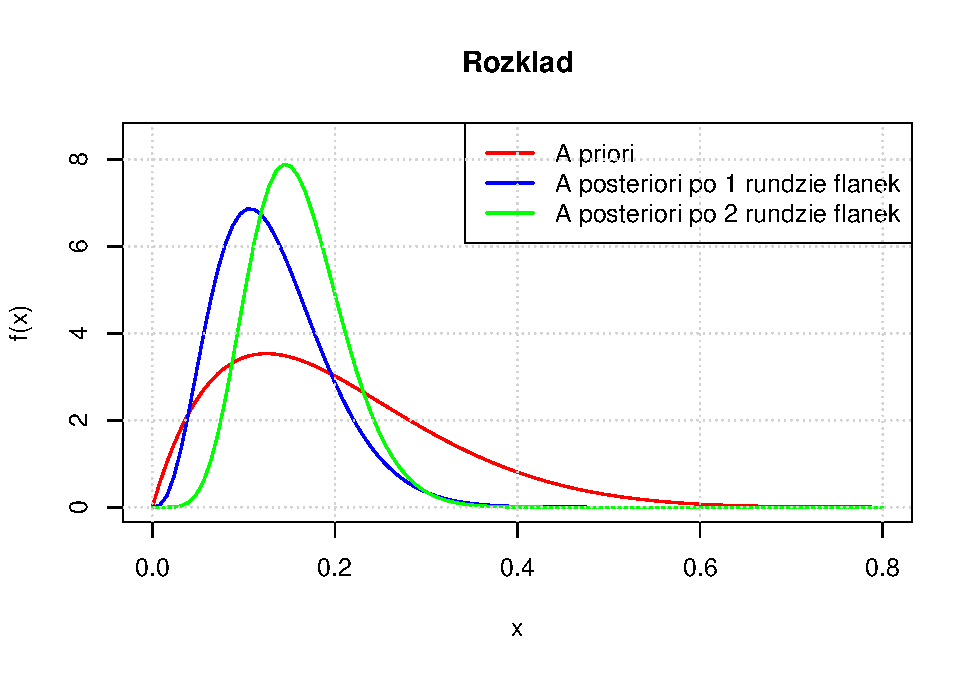
\includegraphics{ADPS_L2_files/figure-latex/unnamed-chunk-12-1.pdf}
Wartość bayesowskiego estymatora \(\hat{p}\) po pierwszej oraz drugiej
rundzie wynosi kolejno 0.1333333, 0.16.

Wariancja dla rozkładu a priori oraz a posteriori po pierwszej oraz
drugiej rundzie flanek wynosi kolejno 0.0145455, 0.0037276, 0.0026353.

Wyznaczone wyniki są minimalnie mniejsze od założonego prawdopodbieństwa
na początku zadania. Na wynik końcówy miało wpływ wiele czynniów takich
jak oświetlenie boiska, wiatr czy ilość wypitego piwa.

\hypertarget{zadanie-4-15-pkt.}{%
\section{Zadanie 4 (1,5 pkt.)}\label{zadanie-4-15-pkt.}}

\hypertarget{treux15bux107-zadania-3}{%
\subsection{Treść zadania}\label{treux15bux107-zadania-3}}

Plik
\href{http://elektron.elka.pw.edu.pl/~mrupniew/adps/fotony.txt}{fotony.txt}
zawiera odstępy między chwilami rejestracji kolejnych fotonów
promieniowania gamma wykonywanymi za pomocą teleskopu kosmicznego
Comptona (CGRO) w roku 1991.

\begin{itemize}
\item
  Wczytaj dane za pomocą komendy scan(`fotony.txt')
\item
  Metodą momentów oraz metodą największej wiarygodności wyznacz estymaty
  parametrów rozkładu gamma odpowiadające zarejestrowanym danym.
  Porównaj wyniki uzyskane dla obu metod.
\item
  Narysuj na jednym wykresie histogram odstępów oraz funkcje gęstości
  rozkładu gamma o parametrach wyestymowanych za pomocą obu metod.
\item
  Metodą bootstrapu parametrycznego wyznacz dla obu metod (momentów oraz
  największej wiarygodności) odchylenia standardowe estymatorów
  parametrów rozkładu gamma (\(\alpha\) i \(\beta\)) oraz ich przedziały
  ufności na poziomie ufności 95\%. Porównaj wyniki uzyskane dla obu
  metod.
\end{itemize}

\begin{Shaded}
\begin{Highlighting}[]
\NormalTok{photons }\OtherTok{=} \FunctionTok{scan}\NormalTok{(}\StringTok{\textquotesingle{}http://elektron.elka.pw.edu.pl/\textasciitilde{}mrupniew/adps/fotony.txt\textquotesingle{}}\NormalTok{)}
\NormalTok{n }\OtherTok{=} \FunctionTok{length}\NormalTok{(photons)}
\NormalTok{quiet }\OtherTok{=} \ConstantTok{TRUE} 
\end{Highlighting}
\end{Shaded}

W celu wyznaczenia wartości parametrów rozkładu gamma \(\alpha\),
\(\beta\) metodą momentów korzystamy z poniższych wzorów:

\[ \hat{\alpha} = \frac{m_{1}^{2}}{m_2-m_{1}^{2}}, \qquad \hat{\beta} = \frac{m_2-m_{1}^{2}}{m_{1}}.\]

\begin{Shaded}
\begin{Highlighting}[]
\NormalTok{m1 }\OtherTok{=} \FunctionTok{mean}\NormalTok{(photons)}
\NormalTok{m2 }\OtherTok{=} \FunctionTok{mean}\NormalTok{(photons}\SpecialCharTok{\^{}}\DecValTok{2}\NormalTok{)}

\NormalTok{alpha\_mom }\OtherTok{=}\NormalTok{ m1}\SpecialCharTok{\^{}}\DecValTok{2}\SpecialCharTok{/}\NormalTok{(m2 }\SpecialCharTok{{-}}\NormalTok{ m1}\SpecialCharTok{\^{}}\DecValTok{2}\NormalTok{)}
\NormalTok{beta\_mom }\OtherTok{=}\NormalTok{ (m2 }\SpecialCharTok{{-}}\NormalTok{ m1}\SpecialCharTok{\^{}}\DecValTok{2}\NormalTok{)}\SpecialCharTok{/}\NormalTok{m1}
\end{Highlighting}
\end{Shaded}

Wartości estymatorów parametrów wyznaczone metodą momentów wynoszą:
\(\hat{\alpha}\) = 1.0655417, \(\hat{\beta}\) = 73.6240637.

W celu wyznaczenia wartości parametru \(\alpha\) oraz \(\hat{\beta}\)
metodą największej wiarygodności, korzystamy z funkcji fitdistr() z
pakietu MASS:

\begin{Shaded}
\begin{Highlighting}[]
\FunctionTok{require}\NormalTok{(MASS)}
\end{Highlighting}
\end{Shaded}

\begin{verbatim}
## Loading required package: MASS
\end{verbatim}

\begin{Shaded}
\begin{Highlighting}[]
\NormalTok{est\_nw }\OtherTok{=} \FunctionTok{fitdistr}\NormalTok{(photons, }\StringTok{\textquotesingle{}gamma\textquotesingle{}}\NormalTok{, }\FunctionTok{list}\NormalTok{(}\AttributeTok{shape=}\DecValTok{1}\NormalTok{, }\AttributeTok{scale=}\DecValTok{1}\NormalTok{), }\AttributeTok{lower=}\DecValTok{0}\NormalTok{)}
\NormalTok{alpha\_nw }\OtherTok{=} \FunctionTok{as.numeric}\NormalTok{(est\_nw}\SpecialCharTok{$}\NormalTok{estimate[}\DecValTok{1}\NormalTok{])}
\NormalTok{beta\_nw }\OtherTok{=} \FunctionTok{as.numeric}\NormalTok{(est\_nw}\SpecialCharTok{$}\NormalTok{estimate[}\DecValTok{2}\NormalTok{])}
\end{Highlighting}
\end{Shaded}

Wartości estymatorów parametrów wyznaczone metodą największej
wiarygodności z wykorzystniem funkcji fitdistr() wynoszą:
\(\hat{\alpha}\) = 1.0519734, \(\hat{\beta}\) = 74.5736621.

\begin{Shaded}
\begin{Highlighting}[]
\FunctionTok{hist}\NormalTok{(photons, }\AttributeTok{breaks =} \DecValTok{50}\NormalTok{, }\AttributeTok{prob =}\NormalTok{ T, }\AttributeTok{col =} \StringTok{\textquotesingle{}red\textquotesingle{}}\NormalTok{, }
     \AttributeTok{xlab =} \StringTok{\textquotesingle{}Odstępy między fotonami\textquotesingle{}}\NormalTok{, }\AttributeTok{ylab =} \StringTok{\textquotesingle{}Częstość występowania\textquotesingle{}}\NormalTok{,}
  \AttributeTok{main =} \StringTok{\textquotesingle{}Histogram odstępów oraz funkcje gęstości }\SpecialCharTok{\textbackslash{}n}\StringTok{ rozkładu gamma\textquotesingle{}}\NormalTok{)}

\FunctionTok{curve}\NormalTok{(}\FunctionTok{dgamma}\NormalTok{(x, }\AttributeTok{shape =}\NormalTok{ alpha\_mom, }\AttributeTok{scale =}\NormalTok{ beta\_mom), }\AttributeTok{add =}\NormalTok{ T, }
      \AttributeTok{col =} \StringTok{\textquotesingle{}blue\textquotesingle{}}\NormalTok{, }\AttributeTok{lwd =} \DecValTok{6}\NormalTok{)}

\FunctionTok{curve}\NormalTok{(}\FunctionTok{dgamma}\NormalTok{(x, }\AttributeTok{shape =}\NormalTok{ alpha\_nw, }\AttributeTok{scale =}\NormalTok{ beta\_nw), }\AttributeTok{add =}\NormalTok{ T,}
      \AttributeTok{col =} \StringTok{\textquotesingle{}green\textquotesingle{}}\NormalTok{, }\AttributeTok{lwd =} \DecValTok{2}\NormalTok{)}

\FunctionTok{grid}\NormalTok{()}

\FunctionTok{legend}\NormalTok{(}\StringTok{\textquotesingle{}topright\textquotesingle{}}\NormalTok{, }\FunctionTok{c}\NormalTok{(}\StringTok{\textquotesingle{}Metoda momentów\textquotesingle{}}\NormalTok{, }\StringTok{\textquotesingle{}Metoda największej wiarygodności\textquotesingle{}}\NormalTok{), }\AttributeTok{col =} \FunctionTok{c}\NormalTok{(}\StringTok{\textquotesingle{}blue\textquotesingle{}}\NormalTok{, }\StringTok{\textquotesingle{}green\textquotesingle{}}\NormalTok{), }\AttributeTok{lwd =} \DecValTok{1}\NormalTok{)}
\end{Highlighting}
\end{Shaded}

\includegraphics{ADPS_L2_files/figure-latex/unnamed-chunk-16-1.pdf}

\begin{Shaded}
\begin{Highlighting}[]
\NormalTok{K }\OtherTok{=} \DecValTok{1000}
\NormalTok{boot\_res\_m }\OtherTok{=} \FunctionTok{replicate}\NormalTok{(K, \{}
\NormalTok{boot\_dane }\OtherTok{=} \FunctionTok{rgamma}\NormalTok{(n, }\AttributeTok{shape =}\NormalTok{ alpha\_mom, }\AttributeTok{scale =}\NormalTok{ beta\_mom)}
\FunctionTok{c}\NormalTok{(}\FunctionTok{mean}\NormalTok{(boot\_dane)}\SpecialCharTok{\^{}}\DecValTok{2}\SpecialCharTok{/}\NormalTok{(}\FunctionTok{mean}\NormalTok{(boot\_dane}\SpecialCharTok{\^{}}\DecValTok{2}\NormalTok{)}\SpecialCharTok{{-}}\FunctionTok{mean}\NormalTok{(boot\_dane)}\SpecialCharTok{\^{}}\DecValTok{2}\NormalTok{),(}\FunctionTok{mean}\NormalTok{(boot\_dane}\SpecialCharTok{\^{}}\DecValTok{2}\NormalTok{)}\SpecialCharTok{{-}}\FunctionTok{mean}\NormalTok{(boot\_dane)}\SpecialCharTok{\^{}}\DecValTok{2}\NormalTok{)}\SpecialCharTok{/}\FunctionTok{mean}\NormalTok{(boot\_dane))}
\NormalTok{\} )}

\NormalTok{sd\_alpha\_mom }\OtherTok{=} \FunctionTok{sd}\NormalTok{(boot\_res\_m[}\DecValTok{1}\NormalTok{,])}
\NormalTok{sd\_beta\_mom }\OtherTok{=} \FunctionTok{sd}\NormalTok{(boot\_res\_m[}\DecValTok{2}\NormalTok{,])}
\end{Highlighting}
\end{Shaded}

Odchylenie standardowe dla estymatora wartości alfy wyznaczonej metodą
momentów wynosi 0.033267.

Odchylenie standardowe dla estymatora wartości bety wyznaczonej metodą
momentów wynosi 2.5462664.

\begin{Shaded}
\begin{Highlighting}[]
\NormalTok{lev }\OtherTok{=} \FloatTok{0.95}
\NormalTok{int\_alpha\_mom }\OtherTok{=} \FunctionTok{quantile}\NormalTok{(boot\_res\_m[}\DecValTok{1}\NormalTok{,], }\FunctionTok{c}\NormalTok{((}\DecValTok{1}\SpecialCharTok{{-}}\NormalTok{lev)}\SpecialCharTok{/}\DecValTok{2}\NormalTok{,(}\DecValTok{1}\SpecialCharTok{+}\NormalTok{lev)}\SpecialCharTok{/}\DecValTok{2}\NormalTok{))}
\NormalTok{int\_beta\_mom }\OtherTok{=} \FunctionTok{quantile}\NormalTok{(boot\_res\_m[}\DecValTok{2}\NormalTok{,], }\FunctionTok{c}\NormalTok{((}\DecValTok{1}\SpecialCharTok{{-}}\NormalTok{lev)}\SpecialCharTok{/}\DecValTok{2}\NormalTok{,(}\DecValTok{1}\SpecialCharTok{+}\NormalTok{lev)}\SpecialCharTok{/}\DecValTok{2}\NormalTok{))}
\end{Highlighting}
\end{Shaded}

Granice 95 \% przedziału ufności dla estymatora wartości alfa
wyznaczonej metodą momentów wynoszą: 1.0049924, 1.1318915.

Granice 95 \% przedziału ufności dla estymatora wartości bety
wyznaczonej metodą momentów wynoszą 68.6374108, 78.6386081.

\begin{Shaded}
\begin{Highlighting}[]
\NormalTok{K }\OtherTok{=} \DecValTok{1000}
\NormalTok{boot\_res\_nw }\OtherTok{=} \FunctionTok{replicate}\NormalTok{(K, \{}
\NormalTok{boot\_dane }\OtherTok{=} \FunctionTok{rgamma}\NormalTok{(n, }\AttributeTok{shape =}\NormalTok{ alpha\_nw, }\AttributeTok{scale =}\NormalTok{ beta\_nw)}
\FunctionTok{c}\NormalTok{(}\FunctionTok{mean}\NormalTok{(boot\_dane)}\SpecialCharTok{\^{}}\DecValTok{2}\SpecialCharTok{/}\NormalTok{(}\FunctionTok{mean}\NormalTok{(boot\_dane}\SpecialCharTok{\^{}}\DecValTok{2}\NormalTok{)}\SpecialCharTok{{-}}\FunctionTok{mean}\NormalTok{(boot\_dane)}\SpecialCharTok{\^{}}\DecValTok{2}\NormalTok{),(}\FunctionTok{mean}\NormalTok{(boot\_dane}\SpecialCharTok{\^{}}\DecValTok{2}\NormalTok{)}\SpecialCharTok{{-}}\FunctionTok{mean}\NormalTok{(boot\_dane)}\SpecialCharTok{\^{}}\DecValTok{2}\NormalTok{)}\SpecialCharTok{/}\FunctionTok{mean}\NormalTok{(boot\_dane))}
\NormalTok{\} )}

\NormalTok{sd\_alpha\_nw }\OtherTok{=} \FunctionTok{sd}\NormalTok{(boot\_res\_nw[}\DecValTok{1}\NormalTok{,])}
\NormalTok{sd\_beta\_nw }\OtherTok{=} \FunctionTok{sd}\NormalTok{(boot\_res\_nw[}\DecValTok{2}\NormalTok{,])}
\end{Highlighting}
\end{Shaded}

Odchylenie standardowe dla estymatora wartości alfy wyznaczonej metodą
największej wiarygodności wynosi 0.034518.

Odchylenie standardowe dla estymatora wartości bety wyznaczonej metodą
największej wiarygodności wynosi 2.6866903.

\begin{Shaded}
\begin{Highlighting}[]
\NormalTok{lev }\OtherTok{=} \FloatTok{0.95}
\NormalTok{int\_alpha\_nw }\OtherTok{=} \FunctionTok{quantile}\NormalTok{(boot\_res\_nw[}\DecValTok{1}\NormalTok{,], }\FunctionTok{c}\NormalTok{((}\DecValTok{1}\SpecialCharTok{{-}}\NormalTok{lev)}\SpecialCharTok{/}\DecValTok{2}\NormalTok{,(}\DecValTok{1}\SpecialCharTok{+}\NormalTok{lev)}\SpecialCharTok{/}\DecValTok{2}\NormalTok{))}
\NormalTok{int\_beta\_nw }\OtherTok{=} \FunctionTok{quantile}\NormalTok{(boot\_res\_nw[}\DecValTok{2}\NormalTok{,], }\FunctionTok{c}\NormalTok{((}\DecValTok{1}\SpecialCharTok{{-}}\NormalTok{lev)}\SpecialCharTok{/}\DecValTok{2}\NormalTok{,(}\DecValTok{1}\SpecialCharTok{+}\NormalTok{lev)}\SpecialCharTok{/}\DecValTok{2}\NormalTok{))}
\end{Highlighting}
\end{Shaded}

Granice 95 \% przedziału ufności dla estymatora wartości alfa
wyznaczonego metodą największej wiarygodności wynoszą: 0.9905859,
1.1227342.

Granice 95 \% przedziału ufności dla beta wyznaczonej metodą największej
wiarygodności wynoszą 69.3991909, 79.7145512.

Obie metody wyznaczenia estymatorów parmetru \(\alpha\) oraz
\(\hat{\beta}\) dały nam podobne wyniki, a narysowane funkcje gęstości
pokrywają się. Świadczy to o poprawności obu metod, a tą któą wybierzemy
w naszych obliczeniach, zależy wyłącznie od nas.

\begin{center}\rule{0.5\linewidth}{0.5pt}\end{center}

\end{document}
